\documentclass[
LEEC,			% Use this option to select your DEE degree, options: LEEC, LETI
english,		% Select document language, options: portuguese or english
%draft,	% Uncomment for draft mode (no pictures, no links, overfull hboxes) 
%twocolumn
]{DEEclass}

% Use the 'preamble.tex' file (root folder) do add packages and macros. Keep your main.tex file clean.

% FYI, the following packages are preloaded with the document class:
% longtable, xcolor, graphicx, booktabs, caption, csquotes, hyperref,
% calc, listings, datetime2, siunitx, geometry, enumitem

%%%%%%%%%%%%%%%%%%%%%%%%%%%%%%%%%%%%%%%%%%%%%%%%%%%%%%%%%% extra packages
\usepackage{amsmath}		% the main package in the AMS-LATEX distribution
\usepackage{amsfonts}		% extended set of fonts for use in mathematics
\usepackage{amssymb}		% adds new symbols to be used in math mode
\usepackage{mathrsfs}		% math fonts, e.g., Laplace
\usepackage{float}			% provides the H float modifier option
\usepackage{multirow}		% tables \multirow command
\usepackage{subcaption}		% enables subfigures
\usepackage{lscape}			% for landscape mode
\usepackage{verbatim}		% new verbatim environment, 
\usepackage{multicol}		% enables multicolumns 
\usepackage[intoc, english]{nomencl} % add nomenclature
\makenomenclature
\usepackage{etoolbox}       % used for nomenclature, i guess...
\makeglossaries
\usepackage{wrapfig}        % enable wrapping figures graphics
\usepackage{graphicx}       % enable graphics
\let\cleardoublepage=\clearpage     % delete blank pages
%\begin{comment}...\end{comment}, \verbatiminput


%add extra packages if needed here

%%%%%%%%%%%%%%%%%%%%%%%%%%%%%%%%%%%%%%%%%%%%%%%%%%%%%%%%%% temp packages
\usepackage{lipsum}						% for fake text
%\usepackage[textsize=tiny]{todonotes}   % enable To-do notes, use the option "disable" to hide all notes, usage \todo{}

%\usepackage{draftwatermark}			% prints a watermark overlay, uncomment if needed
%\SetWatermarkText{**DRAFT**}
%\SetWatermarkScale{1}
%\SetWatermarkColor[gray]{0.8}

%%%%%%%%%%%%%%%%%%%%%%%%%%%%%%%%%%%%%%%%%%%%%%%%%%%%%%%%%% settings
\AtBeginDocument{					% Rendered PDF metadata:
\hypersetup{pdftitle=\ttitle} 		% Sets the PDF title to your dissertation title
\hypersetup{pdfauthor=\authorname} 	% Sets the PDF author to your name
}

%%%%%%%%%%%%%%%%%%%%%%%%%%%%%%%%%%%%%%%%%%%%%%%%%%%%%%%%%% user defined macros









	
% \makenomenclature

%%%%%%%%%%%%%%%%%%%%%%%%%%%%%%%% REPORT INFORMATION %%%%%%%%%%%%%%%%%%%%%%%%%%%%%%%%%%%%%

\reporttitle{Example title} % Your report title

\author{Romain Lambert}	% Your name
\studentnumber{0673627662}	% Your student number
\studentemail{1234567@isep.ipp.pt}	% Your student email address  

\advisor{Nome do Orientador}{xxx@isep.ipp.pt}	% Your ISEP advisor name and email
\coadvisor{Nome do Coorientador}{xxx@isep.ipp.pt}	% Your ISEP co-advisor name and email, comment this line if not needed
\company{Nome da Empresa, Lda.}	% The company name where you developed your work, comment this line if not needed
\supervisor{Nome do Orientador da Empresa}{xxx@emailaddress.com} % Your company supervisor name, comment this line if not needed

%%%%%%%%%%%%%%%%%%%%%%%%%%%%%%%%%%%%%%%%%%%%%%%%%%%%%%%%%%%%%%%%%%%%%%%%%%%%%%%%%%%%%%%%%
\begin{document}

\pagestyle{plain} % Default to the plain heading style until the thesis style is called for the body content

\printcoverpage

%%%%%%%%%%%%%%%%%%%%%%%%%%%%%%%%%%% MAINMATTER %%%%%%%%%%%%%%%%%%%%%%%%%%%%%%%%%%%%%%%%%


\include{Chapters/01 - La théorie.tex}
\section{Le Code }
\label{sec:Ch1}

%%%%%%%%%%%%%%%%%%%%%%%%%%%%%%%%%%%% SUBSECTION 1
\subsection{Le cas d'étude - 2D} 
\label{sec:Ch1.1}

On étudie dans un premier temps La fonction de Breukels pour en chercher les optimum. On utilise pour ce faire un code d'optimsiation fournit par la bibliothèque \textbf{aerosandbox} et on se place dans le cas d'optimisation suivant: 
\begin{itemize}
    \item Maximum de $\sum_{\alpha = 0}^{20}\frac{C_L(\alpha)}{C_D(\alpha)} Gaussienne(alpha, center, sigma) $
\end{itemize}

    où $Gaussienne(\alpha, center, \sigma) = e^{-\frac{(center - \alpha)^2}{2\sigma^2}}$ est une Gaussienne permettant d'obtenir une moyenne pondérée. 

\underline{Les résultats sont présentés dans la partie suivante.}
\begin{figure}[H]
    \centering
    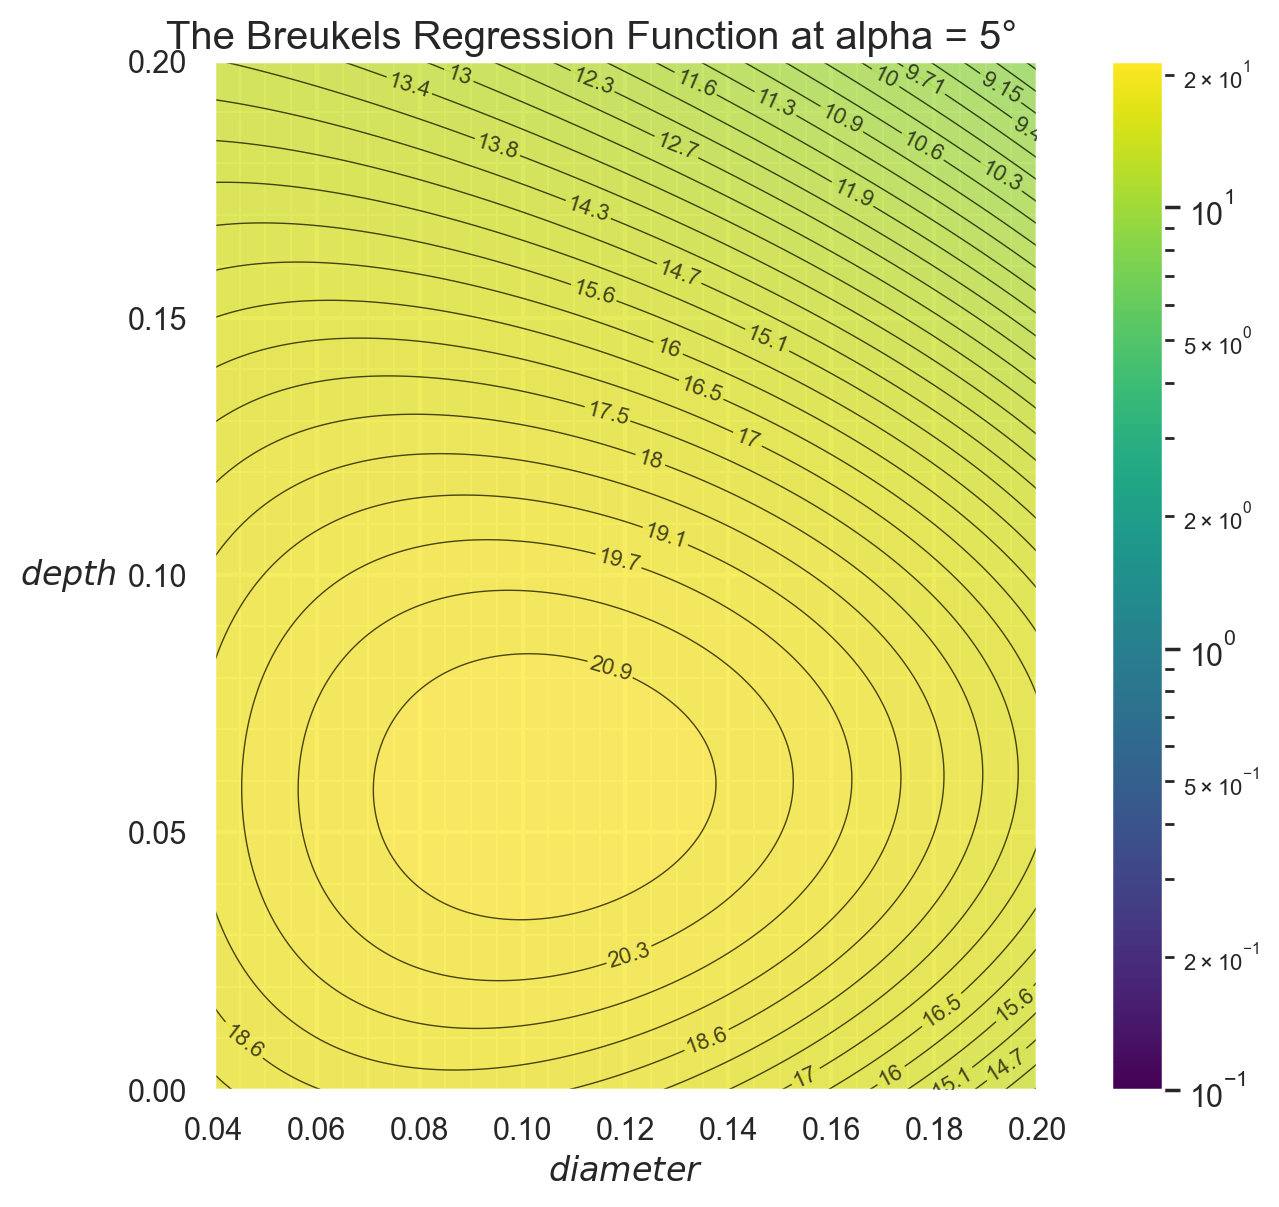
\includegraphics[width=0.5\textwidth]{Pics/breukels.png}  
    \caption{Tracer de $\frac{C_L}{C_D}$ par Régression de Breukels à $\alpha$=5°}
    \label{fig:breukels}
\end{figure}

%%%%%%%%%%%%%%%%%%%%%%%%%%%%%%%%%%%% SUBSECTION 2
\subsection{Le cas d'étude - 3D} 
\label{sec:Ch1.2}

\textbf{L'étude est réalisée à 50 knots}.\\
On se place dans le cas d'étude d'un SK50-VG dont on fait varier le \textbf{diamètre t entre -0.02 et +0.1 et la cambrure k entre -0.1 et 0.1}. \\
    
    On ajoute sur chaque rib les limites suivantes :
    \begin{itemize}
        \item \textbf{le diamètre ne peut pas être inférieur à 0.04}
        \item \textbf{la cambrure ne peut pas être inférieure au demi-diamètre}
    \end{itemize}

    Ainsi, les résultats sont à nuancer : \textbf{une aile avec un certain delta de t ou de k ne veut pas dire que toutes les sections ont été modifiées de ce delta; seules les sections respectant ces critères de minimum énoncés précédemment le sont.}

La loi d'évolution de t et k sur une VG est initialement:  
\begin{itemize}
    \item t : [0.07 0.067 0.065 0.063 0.061 0.06 0.06  0.06 0.06 0.06  0.06  0.06 0.06 0.06  0.06 0.061 0.063 0.065 0.067 0.07]
    \item k : [0.034 0.05 0.0645 0.0686 0.072 0.075 0.08 0.08 0.08 0.08      0.08 0.08 0.08 0.08 0.075 0.072 0.0686 0.0645 0.05 0.034]
\end{itemize}

    A nouveau, on cherche l'optimum dans le problème d'optimisation suivants:
    \begin{itemize}
        \item Maximum de $\sum_{\alpha = 0}^{21}\frac{C_L(\alpha)}{C_D(\alpha)} Gaussienne(alpha, center, sigma) $
    \end{itemize}
    \underline{Les résultats sont présentés dans la partie suivante.}

\begin{figure}[H]
    \centering
    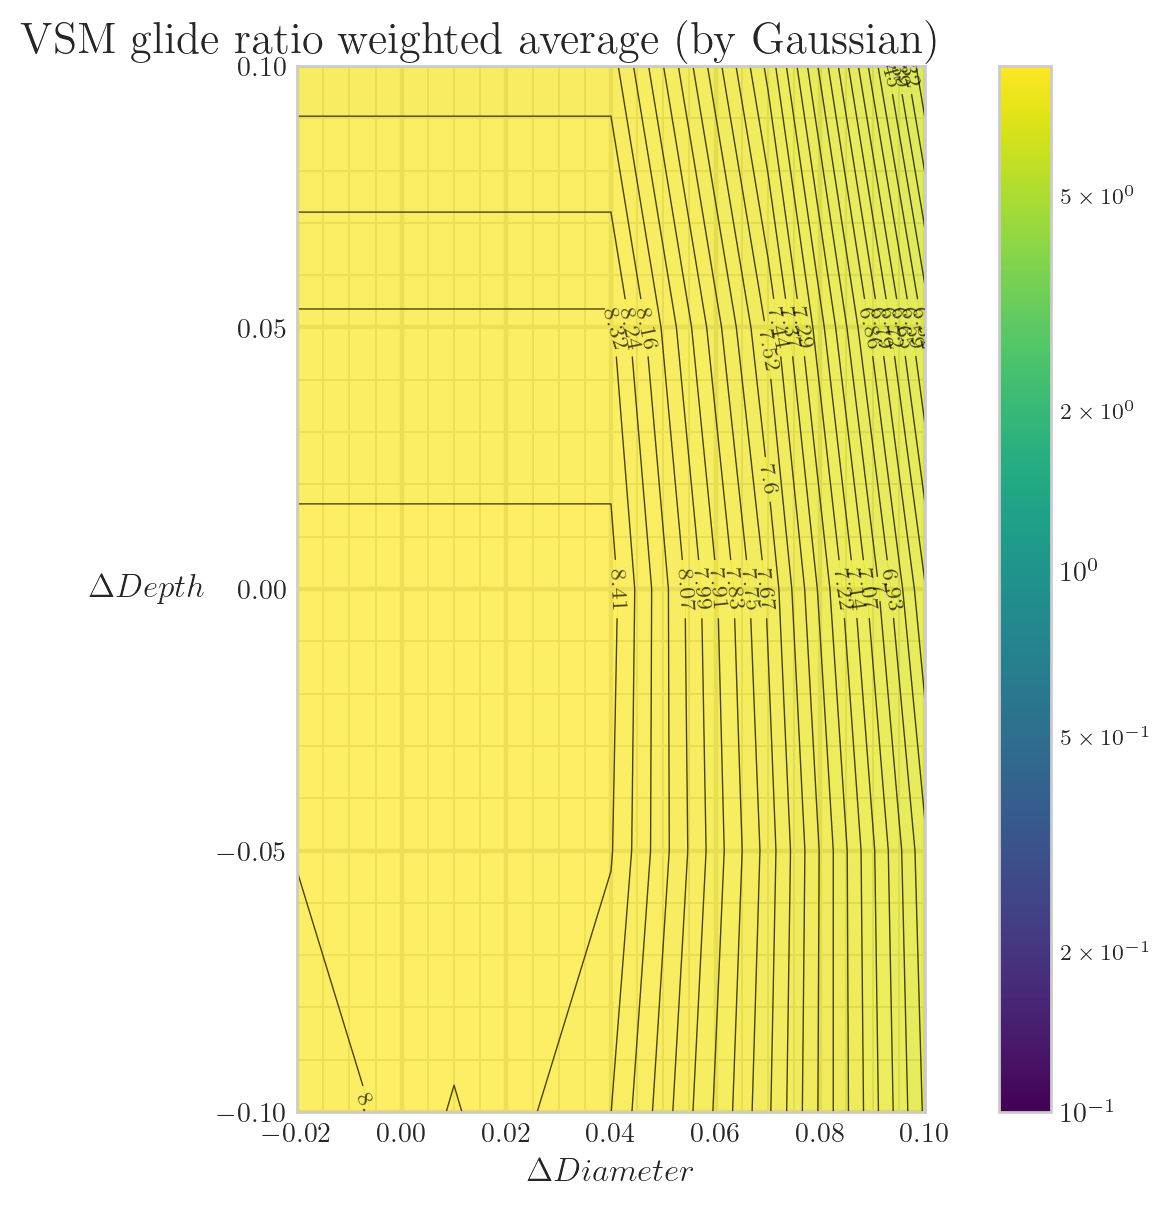
\includegraphics[width=0.5\textwidth]{Pics/vsm.png}  
    \caption{Tracer de $\frac{C_L}{C_D}$ par VSM en faisant varier (t,k)}
    \label{fig:vsm}
\end{figure}
\include{Chapters/03 - Les résultats}
\IEEEpeerreviewmaketitle
\section{ Limites et Etudes Complémentaires}
\label{sec:Ch4}

%%%%%%%%%%%%%%%%%%%%%%%%%%%%%%%%%%%% SUBSECTION 1
\subsection{Limites}
\label{sec:Ch4.1}

Tout d'abord Breukels ne prend en compte que le diamètre et la cambrure maximal d'un profil, \textbf{la position de la cambrure maximale d'un profil n'est donc pas prise en compte}. \\

Ensuite, l'étude réalisée \textbf{ne fait pas intervenir de critère de stabilité.} Il sera sujet par suite d'une telle étude avec les résultats obtenus dans ce papier.\\

De plus, le choix de la fonction objective pour la recherche d'un optimum (moyenne pondérée par une Gaussienne) est peu justifiée. Connaître la valeurs d'un angle d'attaque pour lequel on souhaite optimiser une fonction ( finesse, stabilité, portance...) permettrait d'avoir un résultat plus pertinant. \textbf{Mesurer les angles d'attaques principaux lors des essais kite, peut-être avec l'extended Karmann Filter (EKF)} fournit par Kite Power, permettrait de répondre à ce problème. Le choix de sigma et alpha center dans la Gaussienne sont, eux aussi, criticables.\\

Finalement les fonctions d'optimisation d'Aerosandbox ne sont pas applicables à la VSM. Elles sont cependant utilisées pour optimiser la fonction de Breukels (2 paramètres). \\
Aerosandbox peut aussi représenter et optimiser les profils avec 10 paramètres (Kulfan parameters). Ce n'est pas le sujet de ce papier, cependant c'est une façon différente d'aborder le problème. 

\begin{figure}[H]
    \centering
    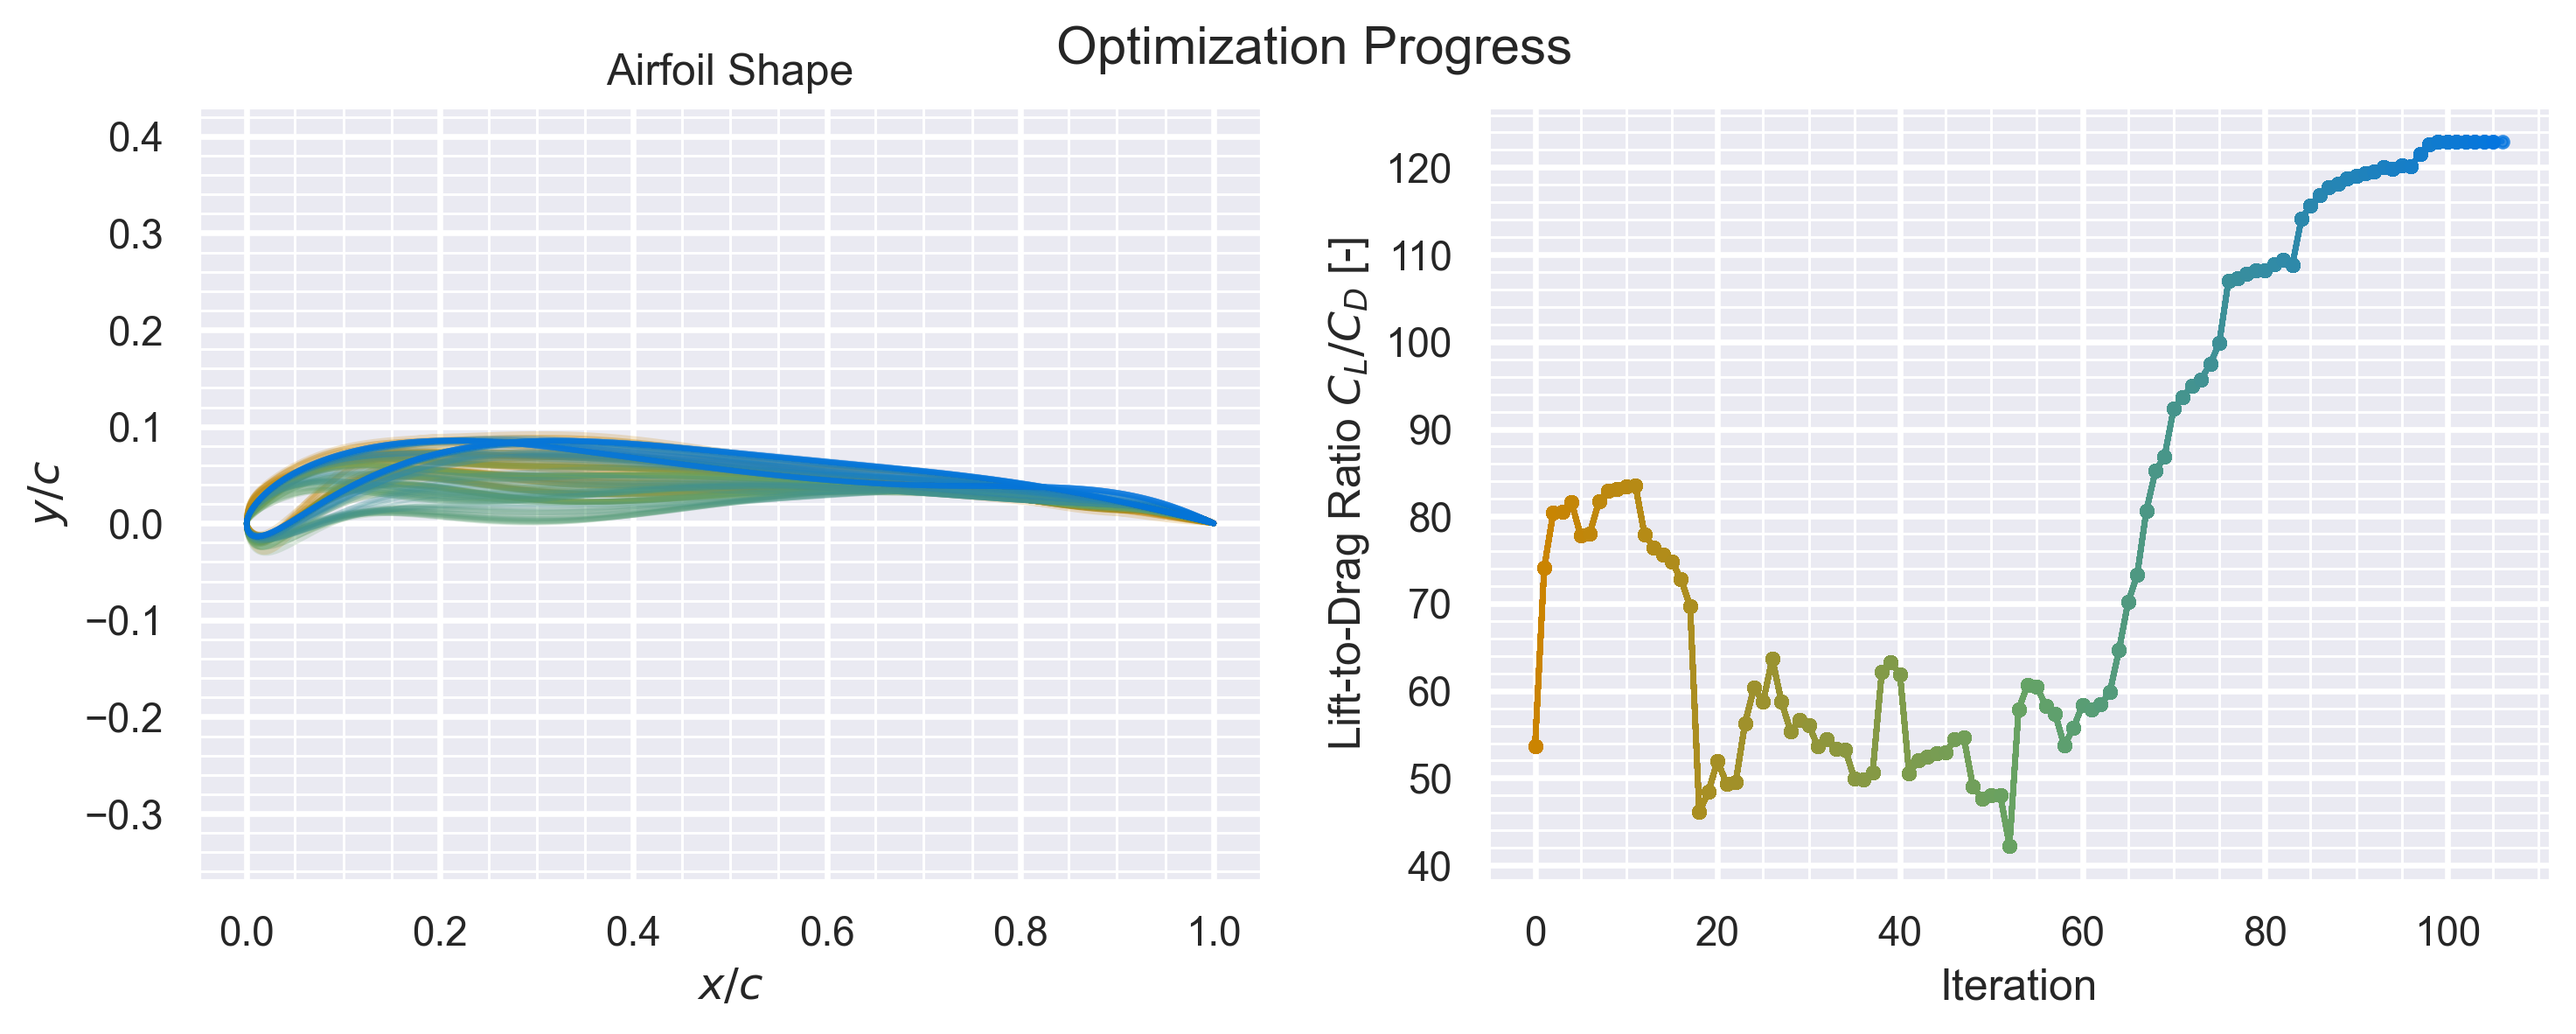
\includegraphics[width=0.5\textwidth]{Pics/optim neuralfoil.png}  
    \caption{Optimisation réalisée avec Aerosandbox sur des profils dis "de Kulfan"}
    \label{fig:kulfan}
\end{figure}

%%%%%%%%%%%%%%%%%%%%%%%%%%%%%%%%%%%% SUBSECTION 2
\subsection{Etudes complémentaires}
\label{sec:Ch4.2}

\begin{itemize}
    \item Comparer sur NeuralFoil et/ou XFoil le profil actuel d’une VG avec le profil optimisé trouvé par OptimXBreukels
    \item Comparer aussi le Cm des 2 profils -> potentiellement conclure sur un profil + performant + stable ?
    \item Créer une base de données d'airfoils polars grâce à Aerosandbox ? qui prend en compte les 3 paramètres (diameter, x depth et depth) et les faire tourner en 2D et ou sur la VSM pour trouver le profil optimal
    \item Faire un chapitre de comparaison des 10m2 classiques vs Hybrid avec profil à caisson, quantifier l'impact de la double peau
\end{itemize}


%%%%%%%%%%%%%%%%%%%%%%%%%%%%%%%%%%%%%%%%%%%%%%%%%%%%%%%%%%%%%%%%%%%%%%%%%%%%%%%%%%%%%%%%% BIBLIOGRAPHY


\end{document}